\documentclass[11pt]{article}

\usepackage[margin=1in]{geometry}
\usepackage[T1]{fontenc}
\usepackage[utf8]{inputenc}
\usepackage{lmodern}
\usepackage{microtype}
\usepackage{amsmath,amssymb}
\usepackage{booktabs}
\usepackage{multirow}
\usepackage{graphicx}
\usepackage[numbers,sort&compress]{natbib}
\usepackage[colorlinks=true,linkcolor=blue,citecolor=blue,urlcolor=blue]{hyperref}
\usepackage{xcolor}

\newcommand{\pp}{\,\%p}   % percentage points

\title{Training-Free Off-Screen Player Imputation for\\Broadcast-Based Spatial Football Analytics}

% TODO(사용자 확인 필요): 실명 + 소속으로 교체. arXiv는 실명 권장.
\author{%
  Nowayfootball\thanks{Independent researcher. Code and data:
  \url{https://github.com/nowayfootball/offscreen-impute}.
  Contact: \texttt{cordelia35794@gmail.com}.}%
}
\date{}

\begin{document}
\maketitle

\begin{abstract}
Spatial football metrics such as pitch control assume access to the positions of
all 22 players, yet the dominant source of positional data --- the broadcast main
camera --- shows only 10--16 of them at any moment. We quantify the resulting
distortion with an open, reproducible benchmark: a simulated broadcast viewport
applied to open full-pitch tracking data (Metrica Sports). Ignoring off-screen
players, the standard practice of video-based game-state-reconstruction (GSR)
pipelines, inflates hidden-zone pitch-control error to 26.9 percentage points and
biases team control share by 13.4 points. We then evaluate a ladder of
\emph{training-free, online} imputation baselines that use only observations from
the match being analysed. The strongest, \emph{role-anchored centroid voting} ---
each visible player votes for the full-team centroid by subtracting its running
role offset, cancelling the viewport-induced subset bias --- cuts hidden-zone
error to 13.3 points and share bias to 4.7 points, consistently across two
matches and viewport widths from 36\,m to 60\,m. In the short-occlusion regime
($\le$9.6\,s) covered by prior learned imputers, our training-free method reaches
median position error of 3--9\,m, comparable to learned models that additionally
exploit future observations; 57\% of real hidden-player mass, however, lies
beyond that regime, which our benchmark is the first to score. We integrate the
method end-to-end into an open broadcast-video GSR pipeline and show that
imputation changes a downstream possession-quality verdict (Space-Creation
Index) by 15--17 points on real World Cup broadcast clips --- a
decision-relevant magnitude.
\end{abstract}

\section{Introduction}

Video-based game state reconstruction (GSR) turns ordinary broadcast footage into
player coordinates on a common pitch template, promising tracking-level analytics
without stadium hardware~\citep{somers2024soccernet}. But the broadcast main
camera pans and zooms with the ball: in our World Cup broadcast clips, and
consistently across the SoccerNet-GSR literature~\citep{somers2024soccernet,
ochin2025footpass}, only 10--16 of the 22 players are visible in a typical frame.
Team-level spatial metrics --- pitch control~\citep{spearman2017physics,
spearman2018beyond}, space value, block compactness --- are then computed over a
biased subset of players: the team whose defenders sit off-screen silently cedes
control of the hidden half of the pitch, not because of anything that happened on
the pitch, but because of where the camera pointed.

This distortion is routinely acknowledged and rarely measured. The GSR evaluation
protocol itself (GS-HOTA~\citep{somers2024soccernet}) scores only the players
that are visible; what happens to downstream \emph{team-level} metrics when the
invisible remainder is ignored has, to our knowledge, not been quantified on open
data. The one closely related study, DeepMind's Graph
Imputer~\citep{omidshafiei2022}, demonstrated the problem and a learned solution,
but on 105 proprietary Premier League tracking matches, with a bidirectional
model that consumes \emph{future} observations inside 9.6-second windows ---
neither reproducible nor applicable in a strictly online setting.

This paper makes three contributions:

\begin{enumerate}
\item \textbf{A reproducible distortion benchmark.} We simulate a broadcast
viewport (ball-tracking pan with lag, width $W$) over open full-pitch tracking
data and score any imputation policy by hidden-zone pitch-control MAE, team
control-share bias, and hidden-player position error --- metrics defined by the
downstream analytics rather than by trajectory fidelity alone
(Section~\ref{sec:benchmark}).
\item \textbf{A ladder of training-free online baselines}, culminating in
\emph{role-anchored centroid voting} (B4), which halves the hidden-zone control
error and cuts control-share bias to a third of the ignore-policy baseline,
without any training data, future observations, or GPU
(Sections~\ref{sec:ladder}--\ref{sec:results}).
\item \textbf{End-to-end integration} into an open video$\to$GSR$\to$metrics
pipeline, with a case study on real World Cup broadcasts where imputation moves a
possession-quality verdict by a decision-relevant magnitude
(Section~\ref{sec:application}).
\end{enumerate}

Our position is deliberately modest: learned imputers remain preferable when
training data and future context are available. What we establish is (i) how
large the distortion actually is, (ii) a strong training-free floor that any
learned method should beat, and (iii) the first scoring of the long-occlusion
regime ($>$9.6\,s) that prior protocols truncate away --- which turns out to hold
the majority (57\%) of real hidden-player observations.

\section{Related Work}
\label{sec:related}

\paragraph{Learned trajectory imputation.}
The Graph Imputer of \citet{omidshafiei2022} is the closest prior work: a
graph-network variational model trained on 105 proprietary EPL tracking matches,
evaluated with a simulated camera view-cone, and applied to pitch control under
partial observability --- the same problem framing as ours. Two protocol
differences preclude direct numeric comparison, and we analyse them explicitly in
Section~\ref{sec:protocol}: their model is bidirectional (it consumes future
observations within 9.6\,s windows), and occlusions are truncated by the window
length, whereas our setting is strictly online with unbounded occlusions.
MIDAS~\citep{choi2025midas} and related set-transformer imputers represent the
learned state of the art on multi-agent trajectory imputation, including
camera-mask experiments. \citet{penn2025continuous} reconstruct continuous
trajectories from discrete broadcast-derived observations with an LSTM/GNN
model --- an adjacent observation model where sparsity is temporal rather than
spatial.

\paragraph{Ghosting.}
The ghosting line of work~\citep{le2017ghosting, yurko2024nflghosts} generates
counterfactual league-average positions --- where a player \emph{should} have
been --- for coaching evaluation. The goal differs from ours: ghosting evaluates
decisions against a baseline policy, whereas imputation recovers actual
unobserved positions for measurement.

\paragraph{Game state reconstruction.}
SoccerNet-GSR~\citep{somers2024soccernet} defines the task and the GS-HOTA
metric for recovering \emph{visible} players from broadcast video; camera
calibration~\citep{gutierrez2024pnlcalib, falaleev2024keypoints} and multi-object
tracking~\citep{aharon2022botsort} supply the geometry and identity backbone.
FOOTPASS~\citep{ochin2025footpass} reports 9--12 visible players per broadcast
frame and notes imputation as a pipeline necessity, corroborating the
universality of the problem. Our benchmark scores the invisible remainder that
GS-HOTA leaves undefined.

\section{Benchmark}
\label{sec:benchmark}

\paragraph{Data.}
Metrica Sports open tracking data~\citep{metrica2020}: two full matches, all 22
players plus ball at 25\,fps. We use the first halves (45 minutes each) and
evaluate at 5\,fps. Using full-pitch tracking as ground truth lets us compute the
\emph{true} spatial metrics and score any partial-observation policy against
them.

\paragraph{Viewport simulator.}
A virtual main camera pans horizontally following an exponentially smoothed ball
position ($\alpha = 0.06$ per frame at 25\,fps), reproducing the pan lag of a
human camera operator; the visible region is a width-$W$ window spanning the full
pitch height. At $W = 44$\,m the viewport shows 14.6 players on average, matching
our real broadcast clips (10--16 visible) and the 12.8$\pm$3.7 reported
by~\citet{omidshafiei2022}. Sensitivity is reported for
$W \in \{36, 44, 52, 60\}$\,m.

\paragraph{Metrics.}
We score three quantities, chosen to reflect the downstream analytics rather
than trajectory fidelity alone:
\begin{enumerate}
\item \textbf{Hidden-player position error} (m): distance between imputed and
true position, over all (frame, player) pairs where the player is outside the
viewport.
\item \textbf{Pitch-control map MAE}: pitch control is computed on a 3\,m grid
with an arrival-time model and sigmoid contest
function~\citep{spearman2017physics}; we report mean absolute error against the
full-observation control map, over the full pitch and over the \emph{hidden
zone} (grid cells outside the viewport) separately. Control is computed with
zero velocities in all conditions, isolating the effect of imputation from that
of velocity estimation.
\item \textbf{Team control-share bias} (percentage points): absolute error in
the single headline number ``team A controls $x\%$ of the pitch''.
\end{enumerate}

\section{The Imputation Ladder}
\label{sec:ladder}

All methods below are \emph{causal} (no future observations), use only
observations from the current match (no training data), and run in real time on
CPU. Let $V_t$ denote the set of visible players at time $t$, $p_i(t)$ the
position of player $i$, and $\mathrm{off}_i(t)$ a running estimate of player
$i$'s \emph{role offset} --- its displacement from the team centroid.

\begin{description}
\item[B0 --- ignore.] Hidden players are absent from the metric. This is the
current practice of GSR pipelines.
\item[B1 --- last-seen with decay.] Hold the last observed position, blending
toward the visible-team mean with time constant $\tau = 8$\,s.
\item[B2 --- formation anchor.] While player $i$ is visible, store
$\mathrm{off}_i = p_i - \bar{p}_{V}$, its offset from the \emph{visible-team}
centroid. When hidden, place the player at the current visible centroid plus the
stored offset.
\item[B3 --- B2 + EMA offsets + velocity extrapolation.] As B2, with
exponentially averaged offsets and short-gap constant-velocity extrapolation.
Kept as a negative result (Section~\ref{sec:results}).
\item[B4 --- role-anchored centroid voting.] The visible-team centroid
$\bar{p}_{V}$ in B2 is itself biased by the viewport: when the camera points
left, the visible subset sits left of the true team centroid, and every stored
offset inherits that bias. B4 removes it by \emph{voting}: each visible player
proposes the full-team centroid as its position minus its role offset,
\begin{equation}
\hat{c}(t) \;=\; \frac{1}{|V_t|}\sum_{i \in V_t}\bigl(p_i(t) - \mathrm{off}_i(t)\bigr),
\qquad
\mathrm{off}_i(t) \;\leftarrow\; \mathrm{EMA}\bigl[\,p_i(t) - \hat{c}(t)\,\bigr]
\quad (i \in V_t),
\end{equation}
a self-consistent bootstrap: offsets are stored relative to the \emph{voted}
centroid, and the voted centroid is computed from those same offsets
(initialised from the visible mean). Hidden player $j$ is imputed at
$\hat{c}(t) + \mathrm{off}_j$. Because each player's individual viewport bias is
subtracted before averaging, the systematic subset bias cancels rather than
accumulates.
\end{description}

\section{Results}
\label{sec:results}

\begin{table}[t]
\centering
\caption{Imputation ladder at $W = 44$\,m (first halves of both Metrica
matches). Lower is better throughout. B0 has no position error since it places
no players.}
\label{tab:ladder}
\small
\begin{tabular}{lcccccc}
\toprule
& \multicolumn{3}{c}{Game 1} & \multicolumn{3}{c}{Game 2} \\
\cmidrule(lr){2-4}\cmidrule(lr){5-7}
& \shortstack{hidden ctrl\\MAE (\%p)} & \shortstack{share\\bias (\%p)} & \shortstack{median pos.\\err.\ (m)}
& \shortstack{hidden ctrl\\MAE (\%p)} & \shortstack{share\\bias (\%p)} & \shortstack{median pos.\\err.\ (m)} \\
\midrule
B0 ignore        & 26.9 & 13.4 & ---  & 25.6 & 12.5 & ---  \\
B1 last-seen     & 22.1 & 10.6 & 19.6 & 20.0 &  9.5 & 17.9 \\
B2 anchor        & 15.7 &  6.2 & 13.6 & 14.6 &  5.4 & 12.8 \\
B3 +velocity     & 12.8 &  5.7 & 14.6 & 11.8 &  4.6 & 14.0 \\
\textbf{B4 centroid vote} & \textbf{13.3} & \textbf{4.7} & \textbf{11.6} & \textbf{12.2} & \textbf{4.5} & \textbf{10.0} \\
\bottomrule
\end{tabular}
\end{table}

\paragraph{Ladder.}
Table~\ref{tab:ladder} reports the ladder at $W = 44$\,m.
Ignoring off-screen players (B0) leaves a hidden-zone control MAE of
25.6--26.9\pp{} and biases the headline control share by 12.5--13.4\pp{}.
The naive last-seen policy recovers only a quarter of that. The formation anchor
(B2) is the single largest step --- most of a hidden player's position is
explained by ``the team moved, the player kept its role''. Centroid voting (B4)
then removes the viewport subset bias that B2 inherits, and is the best method
on both decision-relevant metrics: position error 10.0--11.6\,m median and share
bias 4.5--4.7\pp{}, one third of B0.

\paragraph{Negative result: velocity extrapolation hurts.}
B3's constant-velocity extrapolation \emph{degrades} position error relative to
B2 (14.0--14.6\,m vs.\ 12.8--13.6\,m). The failure mode is systematic: players
typically leave the viewport moving \emph{outward} (that is why they exit), but
then hold their defensive line rather than continuing; extrapolation keeps
pushing them away. The latest formation snapshot is the better prior. B3's
slight edge on hidden-zone map MAE comes from its EMA anchor component, which B4
retains.

\begin{figure}[t]
\centering
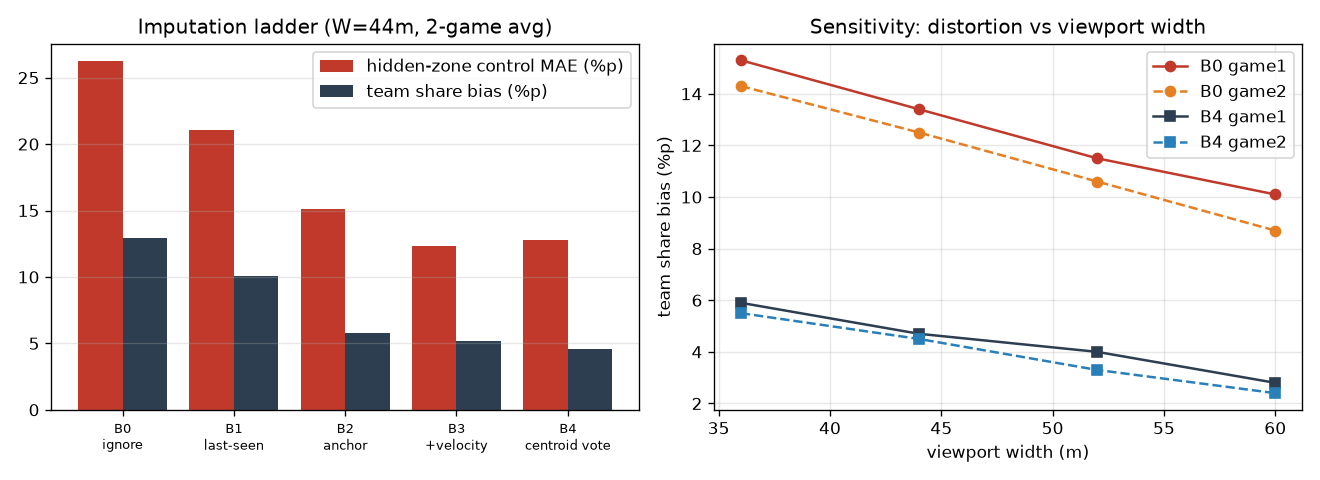
\includegraphics[width=\linewidth]{figures/ladder_sensitivity.png}
\caption{Left: imputation ladder at $W=44$\,m (hidden-zone control MAE and
control-share bias, both games). Right: viewport-width sensitivity --- B4
(solid) vs.\ B0 (dashed) across $W = 36$--$60$\,m. The ordering is monotone and
consistent in both matches; B4's absolute gain is largest in the narrowest
(hardest) viewports.}
\label{fig:ladder}
\end{figure}

\begin{table}[t]
\centering
\caption{Viewport-width sensitivity (game 1 / game 2): hidden-zone control MAE
and control-share bias, B0 vs.\ B4.}
\label{tab:sens}
\small
\begin{tabular}{cccccc}
\toprule
& & \multicolumn{2}{c}{B0 ignore} & \multicolumn{2}{c}{B4 centroid vote} \\
\cmidrule(lr){3-4}\cmidrule(lr){5-6}
$W$ (m) & visible (of 22) & MAE (\%p) & bias (\%p) & MAE (\%p) & bias (\%p) \\
\midrule
36 & 13.0 / 13.1 & 28.9 / 27.6 & 15.3 / 14.3 & 15.6 / 14.1 & 5.9 / 5.5 \\
44 & 14.6 / 14.9 & 26.9 / 25.6 & 13.4 / 12.5 & 13.3 / 12.2 & 4.7 / 4.5 \\
52 & 16.1 / 16.3 & 24.4 / 23.0 & 11.5 / 10.6 & 11.6 / 9.8  & 4.0 / 3.3 \\
60 & 17.2 / 17.4 & 22.8 / 20.6 & 10.1 / 8.7  & 9.5 / 8.0   & 2.8 / 2.4 \\
\bottomrule
\end{tabular}
\end{table}

\paragraph{Sensitivity.}
Table~\ref{tab:sens} and Figure~\ref{fig:ladder} report the sweep over viewport
widths. Across $W = 36$--$60$\,m the method ordering is monotone and consistent
in both matches; B4 reduces share bias to roughly one third of B0 at every
width, with the largest absolute gains in the narrowest (hardest) viewports ---
the method is most valuable exactly when observation is poorest.

\subsection{Occlusion-time stratification and protocol comparison}
\label{sec:protocol}

\begin{table}[t]
\centering
\caption{Observation-protocol comparison with the Graph
Imputer~\citep{omidshafiei2022}. The regimes differ in the two dimensions that
matter most --- temporal information and training data --- so numeric results
are not directly comparable; the stratified analysis below aligns the occlusion
regime.}
\label{tab:protocol}
\small
\begin{tabular}{lll}
\toprule
& Graph Imputer & This work \\
\midrule
Camera model & view-cone $\times$ pitch polygon, ball-led & ball-EMA pan window (width $W$) \\
Visible players & 12.8 $\pm$ 3.7 of 22 & 14.6 of 22 ($W=44$\,m) \\
Temporal structure & bidirectional (sees \emph{future} obs.), & online, causal, \\
& occlusions truncated at 9.6\,s & occlusions unbounded \\
Training data & 105 proprietary EPL matches & none (current match only) \\
Compute & GPU training & CPU, real time \\
\bottomrule
\end{tabular}
\end{table}

Table~\ref{tab:protocol} contrasts the observation protocols. The Graph
Imputer's reported errors benefit from three compounding advantages ---
bidirectional inference over future observations, occlusions truncated to
9.6\,s, and 105 matches of training data --- so we align the comparison by
stratifying B4's position error by occlusion duration:

\begin{center}
\small
\begin{tabular}{lccc}
\toprule
occlusion gap & $\le$2\,s & 2--9.6\,s & $>$9.6\,s \\
\midrule
B4 median position error & 3.3--3.7\,m & 7.2--8.9\,m & $\sim$15.8\,m \\
share of hidden observations & \multicolumn{2}{c}{43\%} & 57\% \\
\bottomrule
\end{tabular}
\end{center}

Within the $\le$9.6\,s regime that the Graph Imputer's protocol scores, a
training-free online method reaches 3--9\,m median error --- competitive with
learned bidirectional models operating with strictly more information. The
majority of real hidden-player mass (57\%), however, lies \emph{beyond} 9.6\,s:
long occlusions of far-side defenders during sustained attacking phases are
precisely where spatial metrics need imputation most, and this regime had not
previously been scored at all. It is also where our absolute errors
($\sim$15.8\,m median) show the remaining headroom, which we expect learned
long-horizon models to attack.

\section{Application: Possession-Quality Verdicts on Real Broadcasts}
\label{sec:application}

\begin{figure}[t]
\centering

\includegraphics[width=\linewidth]{figures/control_panels.png}
\caption{Benchmark visualisation (Metrica, $W = 44$\,m). Left: ground-truth
pitch control from all 22 players. Middle: control from visible players only
(B0) --- the hidden zone (outside the vertical viewport band) is systematically
misassigned. Right: control with B4 imputation (ghost markers) --- the hidden
zone is largely restored without any training data.}
\label{fig:panels}
\end{figure}

To show the distortion is not an artefact of simulation, we integrate B4 into an
open broadcast-video GSR pipeline: PnLCalib-based camera
calibration~\citep{gutierrez2024pnlcalib} with a temporal bridge, BoT-SORT
tracking~\citep{aharon2022botsort}, colour-based team assignment, and shot-change
gating; the pipeline scores GS-HOTA 35.2 on the SoccerNet-GSR test subset
vs.\ the official 26.6 baseline~\citep{somers2024soccernet}. Off-screen players
are rendered as fading ``ghosts'' with role-anchored positions, capped at eleven
per team, and retired when a re-appearing track emerges within 3\,m of a ghost's
prediction.

As a downstream consumer we use a possession-quality metric, the
\emph{Space-Creation Index} (SCI): during a flagged low-threat possession
(``junk possession''), SCI measures whether the possessing team's control of the
attacking third grows while the opponent's advanced control collapses
(positive: the possession creates space even without shots) or nothing moves
(zero or negative: dead possession). On two event-flagged junk-possession
windows from a World Cup broadcast (Morocco--Netherlands), imputation moves the
verdict by a decision-relevant magnitude:

\begin{itemize}
\item Window 1 (0--0, min.\ 12): SCI $+15.6 \to +32.8$. The hidden retreating
defenders, restored by imputation, \emph{amplify} a genuine space-creation
signal that visible-only analysis understates.
\item Window 2 (0--1, min.\ 73): SCI $-10.9 \to +4.7$ --- the verdict class
changes from ``dead junk'' to ``weak progression''.
\end{itemize}

Absent full-pitch ground truth for broadcast footage we make no correctness
claim on real clips; the point is a sensitivity result. Visible-only spatial
verdicts can move by 15--17 SCI points under imputation --- larger than the gap
between verdict classes --- so any pipeline that reports spatial
possession-quality from broadcast video without imputation is reporting, in
part, camera work.

\section{Limitations and Future Work}
\label{sec:limitations}

Identity fragmentation in real GSR output (track fragments; jersey-number OCR
coverage $\approx$45\% in our pipeline) makes roster-aware ghosting approximate
on real video: ghosts anchor to roles, not to verified identities. Appearance
re-identification is the natural next step. The pitch-control model is
velocity-free here to isolate the imputation effect; velocity-aware control with
imputed velocities is open, and our negative result on extrapolation suggests it
is not trivial. The benchmark uses two matches from a single provider; more
matches and leagues would tighten the estimates, though the effect sizes are
large and consistent across both matches and all viewport widths. Finally,
learned imputers remain preferable when future context and training data are
available --- our contribution is the strong training-free floor, the harsher
online/long-occlusion benchmark, and the downstream-metric framing.

\section{Reproducibility}
\label{sec:repro}

All experiments run on CPU with open data (Metrica Sports sample
data~\citep{metrica2020}) and open code; the benchmark, the imputation ladder,
the figures, and the exact commands are available at
\url{https://github.com/nowayfootball/offscreen-impute}. Total compute cost of
every experiment in this paper: \$0.

\bibliographystyle{plainnat}
\bibliography{refs}

\end{document}
